% Created 2014-02-27 Thu 13:55
\documentclass[11pt]{report}
\usepackage[utf8]{inputenc}
\usepackage[T1]{fontenc}
\usepackage{fixltx2e}
\usepackage{graphicx}
\usepackage{longtable}
\usepackage{float}
\usepackage{wrapfig}
\usepackage{rotating}
\usepackage[normalem]{ulem}
\usepackage{amsmath}
\usepackage{textcomp}
\usepackage{marvosym}
\usepackage{wasysym}
\usepackage{amssymb}
\usepackage{hyperref}
\tolerance=1000
\usepackage{minted}
\usepackage[bibstyle=numeric,citestyle=authoryear,backend=biber]{biblatex}
\addbibresource{bibliography.bib}
\usepackage[]{hyperref}
\hypersetup{hidelinks}
\usepackage[]{nomencl}
\author{Volker Strobel}
\date{\today}
\title{Knowledge Engineering Tools for Planning in PDDL - Syntax Highlighting, Task Generation and Plan Visualization and Execution - an extensible framework}
\hypersetup{
  pdfkeywords={},
  pdfsubject={},
  pdfcreator={Emacs 24.3.1 (Org mode 8.2.5h)}}
\begin{document}

\maketitle
\tableofcontents

\begin{abstract}
Automated planning and scheduling blazes a trail for artificial
intelligent behavior. PDDL, a planning language widely used for AI
task specifications requires extensive knowledge engineering effort.
After giving an overview of PDDL syntax and planning basics, a plug-in
(including syntax highlighting) for the code editor Sublime Text and
related editors will be given. A type diagram generator will be
presented that supports modeling of the environment. The usability of
these tools will be evaluated by subjects without prior knowledge in
PDDL. By the use of these tool, the average modeling time of a shorter
task specification could be improved by \ldots{} percent and the error rate
could be reduced from \ldots{} to \ldots{} . Furthermore, this thesis will
present approaches for the automatic generation of task specifications
and provide a basic interface between the functional programming
language Clojure and PDDL. The proposed tools can assist knowledge
engineers in the design process.

\url{https://www.ece.cmu.edu/~koopman/essays/abstract.html}
\end{abstract}
\chapter{Introduction}
\label{sec-1}
\begin{center}
\fbox{
\begin{minipage}[c]{.6\textwidth}
TODO:

\rule[.8em]{\textwidth}{2pt}

\begin{itemize}
\item Scope of the article (What did I miss out, what is included?)
\item Name Tools and provide found possibilities and limitations
\item Motivation: Why is this article interesting?
\item Structure of the article
\item Review of relevant literature? Note: I can review the relevant
literature and related work in the related chapter, if this is
convenient
\item Planning Architecture - 3 Tier Architecture
\item ICAPS
\item Handicapped people -> Planning Interaction
\item Why is something interesting? -> reasons! (and not because it does
not exist yet)
\end{itemize}
\end{minipage}
}
\end{center}

Knowledge engineering (KE), that means representing world information
in a computer system, is the crucial step for utilizing AI planning
system to solve problems. By definition, it requires an expert that
knows the underlying syntax and models the information manually. This
process is naturally error-prone and time-consuming. While planning
system are improving steadily, the main work for useful systems lies
on the representing language. The Planning Domain Definition Language
(PDDL) \parencite{mcdermott1998pddl} allows for a standardized way of
specifying planning tasks. While on the one hand, recent PDDL extensions
\parencite{fox2003pddl2,kovacs2011bnf} extended the expressiveness of
PDDL and tackle a route for real-world applications, they also demand
a higher level of knowledge and attention of the knowledge engineer.
Several approaches to shift the modeling process from a text based
'programming paradigm' to a user-friendly graphical design tool exist,
however, they also arouse drawbacks: limited functionality,
expenditure of time, editing difficulty, to name a few. As in other
computer languages, so far, there is no real way around diving into
the 'code paradigm'. 
This thesis will, after introducing the basic terms and definitions of
PDDL, focus on the software support for knowledge engineers. A package
for the text and source code editor Sublime Text (ST) will be
introduced, that provides syntax highlighting and PDDL templates. And
the functionality is transferred to a on-line editor with instant access. 

Planning is one the the classic Artificial Intelligence (AI) tasks.
The main focus of this thesis is about real world applications and the
development of handy tools that support (and partially automatize) the
planning process. 
\chapter{Related Work}
\label{sec-2}
\section{PDDL Studio}
\label{sec-2-1}
\section{VISPlan}
\label{sec-2-2}

\section{Emacs PDDL Mode}
\label{sec-2-3}

\section{itSimple}
\label{sec-2-4}
\chapter{Planning Basics and PDDL}
\label{sec-3}
\begin{center}
\fbox{
\begin{minipage}[c]{.6\textwidth}


\rule[.8em]{\textwidth}{2pt}

\begin{itemize}
\item Brief summary at start
\item Start with a paragraph that describes the context
\item Very interesing for basics of PDDL:
\item \url{http://www.ida.liu.se/~TDDC17/info/labs/planning/writing.html}
\item Konstruktionsanleitung
\item Propositionale Logic -> Articifial Intelligence a Modern Approach
\item To insert somewhere:
\begin{itemize}
\item It should be mentioned, that almost no planner supports every part
of PDDL. And, additionally, the quality of error messages is very
diversified. While some simple state: error occured, other list the
problem and the line.
\end{itemize}
\end{itemize}
\end{minipage}
}
\end{center}


Introduction to planing:
\url{http://books.google.de/books?id=eCj3cKC_3ikC&printsec=frontcover&dq=automated+planning&hl=en&sa=X&ei=3wgNU5fQIcHx4gSTsoDABA&redir_esc=y#v=onepage&q=automated%20planning&f=false}

AI planning describes \ldots{}

A planner and use the generated solution file (\emph{plan}).

PDDL was first described in PDDL-the planning domain definition
language (1998) and has been in constant development since then.
This thesis makes use of \textcite{pddl3.1} if not otherwise stated. 

PDDL planning task specifications are composed of two separate text files:

\begin{itemize}
\item Domain file: description of general types, predicates, functions
and actions -> uninstanciated problem independent
\item Problem file: description of a concrete problem environment -> instance specific
\end{itemize}

This separation allows for an intuitive process of task modeling:
While general instances are described in the domain file, specific
instances of problems are created in the problem files.

\begin{figure}[htb]
\centering
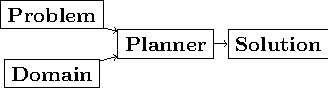
\includegraphics[width=.9\linewidth]{../img/pddl-workflow.pdf}
\caption{\label{fig:workflow}PDDL Planning workflow}
\end{figure}

These two files shell be investigated further in the following
sections.

\section{Format of the Domain File}
\label{sec-3-1}
Domain files have a strict format: All keyword arguments must appear
in the order specified in the manual (an argument may be omitted) and
just one PDDL definition (of a domain, problem, etc.) may appear per
file. \cite[6]{fox2003pddl2}.

\begin{center}
\fbox{
\begin{minipage}[c]{.6\textwidth}


\rule[.8em]{\textwidth}{2pt}

Include simple domain -> \LaTeX{}
Include simple problem -> \LaTeX{}
Include simple plan -> not yet in \LaTeX{}
\end{minipage}
}
\end{center}

\subsection{Define}
\label{sec-3-1-1}
Every domain file start with (define (domain <domainName>) \ldots{}) where,
<domainName> can be any string
\subsection{Requirements}
\label{sec-3-1-2}
The requirements part is not a mandatory part of a PDDL domain file.
However, as most planners only support a subset of PDDL they are
useful for determining if a planner is able to act on a given problem.
They are declared by the (:requirements \ldots{}) part. Some often used
requirements include \ldots{}
\subsection{Types}
\label{sec-3-1-3}

If order to be able to use types in a domain file, the
requirement :typing should be declared.

In order to assign to assign categories of objects, PDDL allows for
type definitions. Like that, parameters in actions can be typed, as
well as arguments in predicates, functions [extra source!]. Later, in
the problem file, objects will be assigned to types, like objects to
classes in Object Orientated Programming (OOP). Adding to the
(:requirement \ldots{}) part of the file guarantees, that typing can be
correctly used. Strips (no types) vs ADL (types).


\subsection{Functions}
\label{sec-3-1-4}
Functions are not supported by many planners (source!) and, before
PDDL 3.1 they could only be modeled as 

It is notable that before PDDL 3.0 the keyword functors was used instead
\subsection{Actions}
\label{sec-3-1-5}
PDDL 3.1 supports two types of actions: durative-action and the
'regular' action.
\section{Format of the Problem File}
\label{sec-3-2}
\section{Format of the Solution File (Plan)}
\label{sec-3-3}
\section{Planning Process}
\label{sec-3-4}
\chapter{Software Engineering Tools for AI Planning}
\label{sec-4}
\begin{center}
\fbox{
\begin{minipage}[c]{.6\textwidth}


\rule[.8em]{\textwidth}{2pt}

\begin{itemize}
\item PDDL type hierarchy and object instantiation to UML / TikZ, store
predicates (and action?) in same box as type
\item Research Knowledge Engineering in Planning
\item Human Computer Interaction
\begin{itemize}
\item \url{http://hci.waznelle.com/checklist.php}
\end{itemize}
\item Write Tiago (itSimple) regarding PDDL -> UML (and knowledge
engineering in general
\item ICKEPS (International Competition on Knowledge Engineering for
Planning and Scheduling)
\item Orient on "How to Design Classes"
\end{itemize}
\end{minipage}
}
\end{center}

\section{Statement of Problem}
\label{sec-4-1}
Writing and maintaining PDDL files can be time-consuming and
cumbersome \textcite{li2012translating}. So, the following development
tools shell support and facilitate the PDDL task design process and
reduce potential errors.

Below, methods are presented for

\begin{description}
\item[{Syntax Highlighting and Code Snippets}] Environment for Editing
PDDL files
\item[{Class Diagram Generator}] The automation of the PDDL task design process. File
input and output and dynamic generation (design level)
\item[{Human Planner Interaction}] An interactive PDDL environment: speech synthesis and
recognition.
\item[{Domain Generator}] Mathematical limitations (design level)
\end{description}
\section{Syntax Highlighting and Code Snippets}
\label{sec-4-2}
\label{sec:syntax}


Writing extensive domain and problem files is a cumbersome task:
longer files can get quickly confusing. Therefore, it is convenient to
have a tool that supports editing these files. Syntax highlighting
describes the feature of text editors of displaying code in different
colors and fonts according to the category of terms (source: Wiki). A
syntax highlighting plug-in for the text and source code editors
\textcite{sublimetext2} and \textcite{sublimetext3} is proposed and
transferred to the on-line text editor Ace are used to implement this
feature, as ST Syntax Highlighting files can easily be converted to
Ace Files. 

For Mac user, TextMate (TM) is very similar to ST and the syntax
highlighting file can be used there, too. Besides, the general
principles (e.g. regular expressions) outlined here, apply to most of
other editors as well.  

\subsection{Implementation}
\label{sec-4-2-1}
ST syntax definitions are written in property lists in the XML format. 

The syntax definition is implemented by the use of the ST plug-in \textcite{aaapackagedev}. So, the definitions can be
written in YAML in converted to Plist XML later on. AAAPackageDEV provides the
following features:

\begin{quote}
AAAPackageDev is a Sublime Text 2 and 3 plug-in
that helps to create and edit syntax definitions, snippets,
completions files, build systems and other Sublime Text extensions.
\end{quote}

By means of Oniguruma regular expressions \parencite{kosako}, scopes are
defined, that determine the meaning of the PDDL code block. The scope naming
conventions mentioned in the \citetitle{textmate} are applied here. By the means
of the name, the colors are assigned. Different ST themes
display different colors (not all themes support all naming conventions).

The syntax highlighting is intended for PDDL 3.1, but is downward
compatible, as previous versions are subsets of later versions.
\begin{center}
\fbox{
\begin{minipage}[c]{.6\textwidth}
Are later versions really subsets?

\rule[.8em]{\textwidth}{2pt}

nil\end{minipage}
}
\end{center}
Like that, the PDDL file is parsed 
\begin{center}
\fbox{
\begin{minipage}[c]{.6\textwidth}
Is it really parsed, or are just parts highlighted?

\rule[.8em]{\textwidth}{2pt}

nil\end{minipage}
}
\end{center}
into different parts. 
\subsection{Usage and Customization}
\label{sec-4-2-2}
By using ST as editor, language independent ST features are supported, like auto
completion, code folding and column selection, described in the
Sublime Text 2 Documentation.

To enable syntax highlighting and code snippets, the files of the
repository have to be placed in the ST packages folder. The first part
of the PDDL.YAML-tmlanguage describes the parts of the PDDL task that
should be highlighted. By removing (or commenting) include statements,
the syntax highlighter is adjustable the user's need.

By default, all scopes are included.

\begin{enumerate}
\item Related Work
\label{sec-4-2-2-1}
\begin{enumerate}
\item PDDL Studio
\label{sec-4-2-2-1-1}
PDDL Studio \parencite{plch2012inspect} is an Integrated Development Environment (IDE) for
creating PDDL tasks. 

\item PDDL Mode
\label{sec-4-2-2-1-2}
Announced 2005 in a mailing list entry, PDDL mode supports PDDL 2.2. 
\item itSIMPLE
\label{sec-4-2-2-1-3}

\item Pygments
\label{sec-4-2-2-1-4}
\item ModPlan
\label{sec-4-2-2-1-5}
\begin{itemize}
\item Very interesting: \url{http://www.tzi.de/~edelkamp/modplan/}
\end{itemize}
\end{enumerate}
\end{enumerate}

\subsection{Evaluation}
\label{sec-4-2-3}

\section{Clojure Interface}
\label{sec-4-3}
As PDDL's syntax is inspired by LISP \parencite[64]{fox2003pddl2},
using a LISP dialect for the interface seems reasonable. This thesis
uses Clojure \parencite{hickey2008clojure}, a relatively modern LISP
dialect that runs on the Java Virtual Machine.

In this section, a kitchen domain will be presented, whereby PDDL
structures are presented that will be also useful in other domains. I
will start with a rather simple domain, present possible limitations
and then extend the file by more sophisticated constructs.
\subsection{Functions}
\label{sec-4-3-1}
As functions have a return value, the modeling possibilities
dramatically increase.

\subsection{Numerical Expressiveness}
\label{sec-4-3-2}
One might assume that the distance could be modeled as follows:

\begin{verbatim}
(durative action ...
...
  :duration (= ?duration (sqrt (coord-x )))
...
\end{verbatim}

However, PDDL does only support basic arithmetic operations (+, -, /, *).

An Euclidean distance function that uses the square root would be
convenient for distance modeling and measurement. However, PDDL 3.1
supports only four arithmetic operators (+, -, /, *). These
operators can be used in preconditions, effects
(normal/continuous/conditional) and durations.
\textcite{parkinson2012increasing} describe a workaround for this
drawback. By declaring an action `calculate-sqrt', they bypass the
lack of this function and rather write their own action that makes use
of the Babylonian root method.

\begin{enumerate}
\item Alternative \#1: Only sqrt exists
\label{sec-4-3-2-1}
Assuming that a function sqrt would actually exist, the duration could be modeled as follows:

\begin{verbatim}
:duration (= ?duration 
             (sqrt
              (+
               (*
                (- (pos-x (current-pos))
                   (pos-x ?goal))
                (- (pos-x (current-pos))
                   (pos-x ?goal)))
               (*
                (- (pos-y (current-pos))
                   (pos-y ?goal))
                (- (pos-y (current-pos))
                   (pos-y ?goal))))))
\end{verbatim}
\item Alternative \#2: sqrt and expt exist
\label{sec-4-3-2-2}
Assuming that a function sqrt would actually exist, the duration could be modeled as follows:
\begin{verbatim}
:duration (= ?duration 
             (sqrt
              (+
               (expt
                (- 
                 (pos-x (current-pos))
                 (pos-x ?goal)))
               (expt
                (- 
                 (pos-y (current-pos))
                 (pos-y ?goal))))))
\end{verbatim}

\item Alternative \#3: Calculate distance and hard code it, e.g. (distance table kitchen) = 5.9
\label{sec-4-3-2-3}

\begin{itemize}
\item Distance Matrix
\item \url{http://stackoverflow.com/questions/20654918/python-how-to-speed-up-calculation-of-distances-between-cities}
\item Scipy.spatial.distance (-> Clojure?)
\item Mention that the Taxicab geometry allows different ways that have an equal length
\end{itemize}

Another alternative is to make use of an external helper and, instead
of calculating every entry of the distance matrix. the distance only
if needed, incorporate every possible combination of two locations.
This approach has certainly a major drawback: With an increasing
amount of locations, the number of combinations increases
exponentially. That means, if there are 100 locations, there will be
\begin{center}
\fbox{
\begin{minipage}[c]{.6\textwidth}
TODO: Calculate possibilities

\rule[.8em]{\textwidth}{2pt}

nil\end{minipage}
}
\end{center}
\ldots{} . The native approach would be to iterate over the cities twice
and calculate only the half of the matrix (as it is symmetric, that
mean distance from A to B is the same as the distance from B to A).

\item Alternative \#4: Use the Manhattan distance
\label{sec-4-3-2-4}

Allowing the agent to move only vertically and horizontally would be
that one can use the so called Taxicab geometry (or Manhattan length)
as distance measurement.  In the Kitchen domain, this could be modeled
as follows:

\begin{verbatim}
% => Metric: reduce duration

% dKitchenware.pddl 
\begin{figure}[t]
\inputminted[mathescape, linenos, numbersep=5pt, frame=lines, framesep=2mm]
            {csharp}
            {Code/dKitchenware.pddl}
\caption{The basic kitchenware domain}
\end{figure}
\section
\end{verbatim}

\begin{center}
\fbox{
\begin{minipage}[c]{.6\textwidth}
TODO:

\rule[.8em]{\textwidth}{2pt}

TODO Human Planner Interaction
\end{minipage}
}
\end{center}
\end{enumerate}
\subsection{PDDL Parsing}
\label{sec-4-3-3}

\section{Type Diagram Generator}
\label{sec-4-4}
\begin{center}
\fbox{
\begin{minipage}[c]{.6\textwidth}


\rule[.8em]{\textwidth}{2pt}

Add actions to the Type Diagram?
\end{minipage}
}
\end{center}

Types play a major role in the PDDL design process: they are involved,
besides their definition, in the constants, predicates and actions
part. So, a fine grasp of their hierarchy, as well as their involved
predicates becomes handy and assists the KE in the planning process. 

\chapter{Analysis}
\label{sec-5}
\section{Participants}
\label{sec-5-1}
Ten non-paid students (six female) took part in the experiment. All
had knowledge about LISP syntax, but neither one had faced PDDL prior
to this study. 
\section{Material}
\label{sec-5-2}
The usability of the Syntax Highlighter (see \ref{sec:syntax}) and the Type
Diagram Generator (see \texttt{Type Diagram Generator}) were
tested.
\section{Design}
\label{sec-5-3}

The participants had to 

\section{Procedure}
\label{sec-5-4}
\chapter{Discussion and Outlook}
\label{sec-6}
\chapter{Bibliography}
\label{sec-7}
\printbibliography

\chapter{Appendix}
\label{sec-8}
\(\alpha\)
% Emacs 24.3.1 (Org mode 8.2.5h)
\end{document}
